%!TEX TS-program = xelatex
%!TEX encoding = UTF-8

% Template for the class file AJbook, originally designed for Chinese book ``代数学方法''.
% Copyright 2018  李文威 (Wen-Wei Li).
% Permission is granted to copy, distribute and/or modify this
% document under the terms of the Creative Commons
% Attribution 4.0 International (CC BY 4.0)
% http://creativecommons.org/licenses/by/4.0/

% 使用自定义的文档类 AJbook.cls. 自动载入 xeCJK. 需要额外档案如下:
% font-setup-open.tex, coverpage.tex, titles-setup.tex, mycommand.sty, myarrows.sty
% 文档类选项 (key/val 格式):
% draftmark = true (未定稿, 底部显示日期) 或 false (成品), 默认 false,
% colors = true (链接带颜色无框) 或 false (黑色无框), 默认 true,
% traditional = true (繁体中文) 或 false (简体中文), 默认 false,
% coverpage = 封面档档名, 默认为空 (此时不制作封面), 一般是 .tex 档, 若为 *.pdf 的形式则直接引入 PDF 页面.
% fontsetup = 字体设置档档名,
% titlesetup = 章节格式设置档名.

% 注意: 如果文中未使用 \cite 和 \index 命令, 则可能报错.

% 需动用 imakeidx + xindy (两份索引), biblatex + biber (书目). 
% 索引用土法进行中文排序: 如 \index{zhongwen@中文} 等.
\documentclass[
	draftmark = true,   % 草稿模式下, 每页底部将打印相关版本信息.
%	traditional = true,
%	colors = false,
%	coverpage = coverpage.tex,
%	coverpage = coverpage.pdf,
%   geometry = b5,    % 版面设置, 目前仅容许 a4, b5, 默认 b5, 其它字串则不作自动设置.
	fontsetup = font-setup-open.tex,
	titlesetup = titles-setup.tex
]{AJbook}

% 可以修改章节编号的深度
% \setcounter{secnumdepth}{3}

% 必要时仅引入部分档案
% \includeonly{}

% 生成索引: 选用 xindy + imakeidx
\usepackage[xindy, splitindex]{imakeidx}
\makeindex[
	columns=2,
	program=truexindy,
	intoc=true,
	options=-M texindy -I xelatex -C utf8,
	title={名词索引}]	% 名词索引

\usepackage[unicode, bookmarksnumbered]{hyperref}	% 启动超链接和 PDF 文档信息所需
% 设置 PDF 文件信息
\hypersetup{
	pdfauthor = {李文威 (Wen-Wei Li)},
	pdftitle = {AJbook 文档类模板},
	pdfkeywords = {Template},
	CJKbookmarks = true}

% 用 bibLaTeX 生成参考文献, 作为示例, 这里引入的是 Al-jabr.bib.
% 载入书目库: 文档类业已引入 biblatex + biber
\addbibresource{Al-jabr.bib}

% 增加表格高度
\renewcommand*\arraystretch{1.5}

% 自订公式的编号 (非必要)
\numberwithin{equation}{section}
\renewcommand{\theequation}{\thesection--\arabic{equation}}

% 自订 figure 的编号 (非必要)
%\numberwithin{figure}{section}
%\renewcommand{\thefigure}{\thechapter--\arabic{figure}}

% 自订 table 的编号 (非必要)
%\numberwithin{table}{section}
%\renewcommand{\thetable}{\thechapter--\arabic{table}}

\begin{document}
	\frontmatter	% 制作封面和目录.
	% 注意: 为了简化, 本模板不含封面. 请通过文档类的参数进行设置.
	
	\mainmatter		% 正文开始:逐章引入 TeX 代码

	\chapter*{导言}
	\section*{简要说明}
	\paragraph*{旨趣}
	此模板的目的是演示文档类 \textsf{AJbook} 的基本用法. 顾名思义, \textsf{AJbook} 原来是为了《代数学方法》一书量身打造的文档类, 基于 \LaTeX 的标准类 \texttt{book}; 但在设计时容许了一定的弹性, 所以它也能够用来制作基础数学或物理领域的中文专业书籍. 字型和各章节的排版方式可以另外调整, 但为了简单起见, 本模板直接沿用《代数学方法》卷一的设置, 打开草稿模式, 并且不含封面.

	\paragraph*{附记}
	\begin{enumerate}
		\item 此文档类也支持繁体中文.
		\item 文章结构中的``部分''(由 \texttt{\textbackslash part} 命令产生), 各章最后的习题, 附录, 以及图/表索引并不是必要的, 放在这里只是作为演示.
		\item 以下内容仅作测试用途, 无其它意涵.
	\end{enumerate}

	\section*{致谢}
	文档类是从头撰写的, 但排版方式受高等教育出版社的模板启发, 在此表示谢意.

	\vspace{1em}
	\begin{flushright}\begin{minipage}{0.3 \textwidth}
		\begin{tabular}{c}
			{\kaishu 李文威} \\
			2019 年元旦\\
			记于北大理教三层
		\end{tabular}
	\end{minipage}\end{flushright}

	% % % % % % % % % %
	\part{测试}
	\chapter{各种测试}
	各章开头可有说明文字.\footnote{脚注测试} 视情况加入阅读提示.
	\begin{wenxintishi}
		本章 \S\ref{sec:words} 的文字撷取自《明儒学案》, [清] 黄宗羲, 仅作测试之用. 来源于网络, 恐怕多有错漏, 请见谅. \index{huangzongxi@黄宗羲}
	\end{wenxintishi}

	\section{节 (section)}
	关于数学词汇的汉译, 比较全面的参考书是 \cite{ZG}.
	\begin{theorem}[L.\ Euler]
		以下结果是熟知的.
		\begin{equation}\label{eqn:zeta-2}
			\sum_{n=1}^\infty \frac{1}{n^2} = \frac{\pi^2}{6}.
		\end{equation}
		当然, 公式的编号方式可以自订.
	\end{theorem}

	文中可以穿插练习及其提示.
	\begin{exercise}\label{exo:Euler}
		试补全公式 \eqref{eqn:zeta-2} 的证明. \begin{hint} 参看表 \ref{table:B}.\end{hint}
	\end{exercise}

	\begin{itemize}
		\item 已知的其它 $\zeta$ 值包括 $\zeta(4) = \pi^4/90$, $\zeta(6) = \pi^6/945$ 等等.
		\item 一般而言, 对所有正整数 $n$ 都有
		\begin{equation}
			\zeta(2n) = (-1)^{n+1} \underbracket{B_{2n}}_{\text{Bernoulli 数}} \frac{(2\pi)^{2n}}{2(2n)!}.
		\end{equation}
		关于 Bernoulli 数\footnote{脚注再测试}, 请见 \S\ref{sec:B}.
	\end{itemize}

	超链接测试: 请常用 \href{http://mathoverflow.net}{MathOverflow}

	\section{文字测试}\label{sec:words}

	测试 \textsf{description} 环境如下:
	\begin{description}
		\item[明儒学案] 中国第一部完整的学术史著作
		\item[黄宗羲 (1610---1695)] 明末清初思想家、文学家。字太冲,号梨洲,又号南雷。
	\end{description}
	
	\subsection{子节 (subsection)}
	以下测试定义, 定理, 证明等等, 以及文字加粗.
	
	\begin{definition}
		盈天地皆心也,变化不测,不能不万殊。\emph{心无本体,工夫所至,即其本体},故穷理者,穷此心之万殊,非穷万物之万殊也。是以古之君子,宁凿五丁之间道,不假邯郸之野马,故其途亦不得不殊!奈何今之君子,必欲出於一途,使美厥灵根者,化为焦芽绝港。夫先儒之语录,人人不同,只是印我之心体,变动不居,若执定成局,终是受用不得。此无他,修德而后可讲学。今讲学而不修德,又何怪其举一而废百乎?
	\end{definition}

	\subsection*{无编号子节 (subsection*)}
	无编号者不列入目录.
	\begin{proposition}[胡居仁]
		胡居仁字叔心,饶之余干人也。学者称为敬斋先生。弱冠时奋志圣贤之学,往游康斋吴先生之门,遂绝意科举,筑室於梅溪山中,事亲讲学之外,不干人事。久之,欲广闻见,适闽历浙、入金陵,从彭蠡而返。所至访求问学之士,归而与乡人娄一斋、罗一峰、张东白为会於弋阳之龟峰、余干之应天寺。提学李龄、锺城相继请主白鹿书院。诸生又请讲学贵溪桐源书院。淮王闻之,请讲《易》於其府。王欲梓其诗文,先生辞曰:“尚需稍进。”先生严毅清苦,左绳右矩,每日必立课程,详书得失以自考,虽器物之微,区别精审,没齿不乱。
	\end{proposition}

	\subsubsection{次子节 (subsubsection)}
	次子节默认不再编号. 如需编号, 请手动设置 \LaTeX 中标准的 \textsf{secnumdepth} 参数.

	\begin{lemma}[陈献章]\label{prop:chen}
		有明之学,至白沙始入精微。其吃紧工夫,全在涵养。喜怒未发而非空,万感交集而不动,至阳明而后大。两先生之学,最为相近,不知阳明后来从不说起,其故何也?薛中离,阳明之高第弟子也,於正德十四年上疏请白沙从祀孔庙,是必有以知师门之学同矣。罗一峰曰:“白沙观天人之微,究圣贤之蕴,充道以富,崇德以贵,天下之物,可爱可求,漠然无动於其中。”信斯言也,故出其门者,多清苦自立,不以富贵为意,其高风之所激,远矣。
	\end{lemma}
	\begin{proof}
		陈献章字公甫,新会之白沙里人。身长八尺,目光如星,右脸有七黑子,如北斗状。自幼警悟绝人,读书一览辄记。尝读《孟子》所谓天民者,慨然曰:“为人必当如此!”梦拊石琴,其音泠泠然,一人谓之曰:“八音中惟石难谐,子能谐此,异日其得道乎?”因别号石斋。正统十二年举广东乡试,明年会试中乙榜,入国子监读书。已至崇仁,受学於康斋先生,归即绝意科举,筑春阳台,静坐其中,不出阈外者数年。寻遭家难。成化二年,复游太学,祭酒邢让试和杨龟山《此日不再得》诗,见先生之作,惊曰:“即龟山不如也。”扬言於朝,以为真儒复出,由是名动京师。罗一峰、章枫山、庄定山、贺医闾皆恨相见之晚,医闾且禀学焉。归而门人益进。十八年,布政使彭韶、都御史朱英交荐,言“国以仁贤为宝,臣自度才德不及献章万万,臣冒高位,而令献章老丘壑,恐坐失社稷之宝”。召至京,阁大臣或尼之,令就试吏部。辞疾不赴,疏乞终养,授翰林院检讨而归。有言其出处与康斋异者,先生曰:“先师为石亨所荐,所以不受职;某以听选监生,始终愿仕,故不敢伪辞以钓虚誉,或受或不受,各有攸宜。”自后屡荐不起。弘治十三年二月十日卒,年七十有三。先生疾革,知县左某以医来,门人进曰:“疾不可为也。”先生曰:“须尽朋友之情。”饮一匙而遣之。
	\end{proof}

	\paragraph{段落 (paragraph)} 段落一般也不编号.
	\begin{corollary}[吕柟]
		字仲木,号泾野,陕之高陵人。正德戊辰举进士第一,授翰林修撰。逆瑾以乡人致贺,却之,瑾不悦。已请上还宫中,御经筵,亲政事,益不为瑾所容,遂引去。瑾败,起原官。上疏劝学,危言以动之。乾清宫灾,应诏言六事:一、逐日临朝,二、还处宫寝,三、躬亲大祀,四、日朝两宫,五、遣去义子、番僧、边军,六、撤回镇守中官。皆武宗之荒政。不听,复引去。世庙即位,起原官。甲申以修省自劾,语涉大礼,下诏狱。降解州判官,不以迁客自解,摄守事,兴利除害若嗜欲。
	\end{corollary}
	\begin{proof}
		未第时,即与崔仲凫讲於宝邛寺。正德末,家居筑东郭别墅,以会四方学者。别墅不能容,又筑东林书屋。镇守廖奄张甚,其使者过高陵,必诫之曰:“吕公在,汝不得作过也。”在解州建解梁书院,选民间俊秀,歌诗习礼。九载南都,与湛甘泉邹东廓共主讲席,东南学者,尽出其门。尝道上党,隐士仇栏遮道问学。有梓人张提闻先生讲,自悟其非,曾妄取人物,追还主者。先生因为诗云:“岂有征夫能过化,雄山村里似尧时。”朝鲜国闻先生名,奏谓其文为式国中。先生之学,以格物为穷理。及先知而后行,皆是儒生所习闻。而先生所谓穷理,不是泛常不切於身,只在语默作止处验之;所谓知者,即从闻见之知,以通德性之知,但事事不放过耳。大概工夫,下手明白,无从躲闪也。
	\end{proof}

	\begin{remark}
		诸生有言及气运如何,外边人事如何者。曰:“\emph{此都是怨天尤人的心术}。但自家修为,成得个片段,若见用,则百姓受些福;假使不用,与乡党朋友论些学术,化得几人,都是事业,正所谓畅於四肢,发於事业也,何必有官做,然后有事业。” 
	\end{remark}

	\section{字体和大小}
	自带的设定档中定义了中文排版常用的几种字体命令, 可以手动切换. 如表 \ref{table:ziti}.
	\begin{table}[h!]
		\begin{tabular}{ll}
			\texttt{\textbackslash heiti} & {\heiti 黑体} \\
			\texttt{\textbackslash songti} & {\songti 宋体} \\
			\texttt{\textbackslash kaishu} & {\kaishu 楷体} \\
			\texttt{\textbackslash fangsong} & {\fangsong 仿宋}
		\end{tabular}
		\caption{几种字体命令} \label{table:ziti}
	\end{table}

	\emph{注意}: \LaTeX 的精神是尽量让作者专注于内容, 外观则留给模板. 频繁地手动切换字体不是个好主意.
	
	字体大小由标准命令控制, 如表 \ref{table:ziti-size} 所示.

	\begin{table}[h!]
		\begin{tabular}{ll}
			\texttt{\textbackslash tiny} & {\tiny 极高明而道中庸} \\
			\texttt{\textbackslash scriptsize} & {\scriptsize 极高明而道中庸} \\
			\texttt{\textbackslash footnotesize} & {\footnotesize 极高明而道中庸} \\
			\texttt{\textbackslash small} & {\small 极高明而道中庸} \\
			\texttt{\textbackslash normalsize} & {\normalsize 极高明而道中庸} \\
			\texttt{\textbackslash large} & {\large 极高明而道中庸} \\
			\texttt{\textbackslash Large} & {\Large 极高明而道中庸} \\
			\texttt{\textbackslash LARGE} & {\LARGE 极高明而道中庸} \\
			\texttt{\textbackslash huge} & {\huge 极高明而道中庸} \\
			\texttt{\textbackslash Huge} & {\Huge 极高明而道中庸}
		\end{tabular}
		\caption{字体大小效果} \label{table:ziti-size}
	\end{table}

	\section{图片}
	
	本模板采用\emph{知识共享}署名 4.0 国际许可协议进行许可. 点击\href{http://creativecommons.org/licenses/by/4.0/}{链接}查看该许可协议.
	\begin{figure}[h!]\begin{center}
		
\includegraphics{ccby.png}
		\caption{许可协议图片}
	\end{center}\end{figure}

	\section{混排公式 \texorpdfstring{$e^{i\theta} = \cos\theta + i\sin\theta$}{exp itheta = cos theta + isin theta}}
	西文按寻常方式进行排版.
	\begin{quote}
		La connaissance de la misère humaine est difficile au riche, au puissant, parce qu'il est presque invinciblement porté à croire qu'il est quelque chose. Elle est également difficile au misérable parce qu'il est presque invinciblement porté à croire que le riche, le puissant est quelques chose.

		\begin{flushright}\textit{La Pesanteur et la grâce}, Simone Weil\end{flushright}
	\end{quote}

	每章最后可以集中安排习题.
	\begin{Exercises}
		\item 试证......
		\begin{hint}
			请自己做.
		\end{hint}
		\item 试说明在一般的环 $R$ 中
		\begin{enumerate}
			\item 对所有 $x, y \in R$ 皆有 $x + y = y + x$;
			\item 但一般而言
			\[ xy \neq yx. \]
		\end{enumerate}
	\end{Exercises}

	% % % % % % % % % %
	\part{更多测试}
	\chapter[短章名]{这是一个充分长的章名, 强势占用三行没商量.}
	如果章名过长, 可以在目录和天眉以另外设置的短章名显示, 方式和 \LaTeX 的标准文档类 \textsf{book} 相同.

	\section{长度正常的节名}
	复数 $\tau$ 的虚部记为 $\Im(\tau)$. 自然对数记为 $\log$.
	
	\begin{convention}\index{Dedeking $\eta$ 函数}
		本节记 Poincaré 上半平面为
		\[ \mathcal{H} := \left\{ \tau \in \mathbb{C}: \Im(\tau) > 0 \right\}. \]
		按例记 $q := e^{2\pi i \tau}$.	\emph{Dedekind $\eta$ 函数}定义为无穷乘积
		\[ \eta(\tau) := e^{2\pi i \tau/24} \prod_{n=1}^\infty (1 - q^n), \quad \tau \in \mathcal{H}. \]
	\end{convention}
	由分析学常识易见此无穷乘积绝对收敛. 进一步, $\eta$ 在 $\mathcal{H}$ 上全纯无零点; 此外 $\eta$ 的对数导数为
	\[ \frac{\mathrm{d}}{\mathrm{d}\tau} \log \eta (\tau) := \frac{\eta'(\tau)}{\eta(\tau)} = \frac{\pi i}{12} - 2\pi i \sum_{n=1}^\infty \frac{n q^n}{1 - q^n}. \]
	
	\begin{example}
		在右半复平面上定义 $\sqrt{z} := \exp(\log|z| + i\arg(z))$, 其中幅角取 $\arg(z) \in \left[-\frac{\pi}{2}, \frac{\pi}{2}\right]$. 则
		\[ \eta\left( \frac{-1}{\tau} \right) = \sqrt{-i\tau} \cdot \eta(\tau), \quad \tau \in \mathcal{H}. \]
	\end{example}
	\begin{proof}
		应用 Eisenstein 级数 $E_2$ 的性质, 将对数导数 $\frac{\mathrm{d}}{\mathrm{d} \tau} \log\eta(\tau)$ 整理为
		\begin{multline*}
			\frac{\pi i}{12} - 2\pi i \sum_{d \geq 1} \frac{dq^d}{1- q^d} = \frac{\pi i}{12} - 2\pi i \sum_{d \geq 1} \sum_{k \geq 1} d q^{dk} \\
			\stackrel{n := dk}{=} \frac{\pi i}{12} - 2\pi i \sum_{n \geq 1} \sigma_1(n) q^n = \dfrac{\pi i}{12} \cdot E_2(\tau),
		\end{multline*}
		若改为对 $\tau \mapsto \eta(\frac{-1}{\tau})$ 求对数导数, 再应用 $E_2$ 的函数方程, 产物则是
		\[ \tau^{-2} \cdot \frac{\pi i}{12} \cdot E_2\left(\frac{-1}{\tau}\right) = \frac{\pi i}{12} \left(E_2(\tau) + \frac{12}{2\pi i \tau} \right). \]
		对 $\sqrt{-i\tau}$ 求对数导数给出 $\frac{1}{2} \frac{\mathrm{d}}{\mathrm{d}\tau} \log(-i\tau) = \dfrac{1}{2\tau} = \dfrac{\pi i}{12} \cdot \dfrac{12}{2 \pi i \tau}$. 与上式对比即见
		\begin{align*}
			\frac{\mathrm{d}}{\mathrm{d} \tau} \log \eta\left( \frac{-1}{\tau} \right) & = \frac{\mathrm{d}}{\mathrm{d} \tau} \log \sqrt{-i\tau} + \frac{\mathrm{d}}{\mathrm{d} \tau} \log \eta(\tau)  \\
			& = \frac{\mathrm{d}}{\mathrm{d} \tau} \log \left( \sqrt{-i\tau} \cdot \eta(\tau) \right).
		\end{align*}
		故存在 $c \in \mathbb{C}^\times$ 使得 $\eta\left(\frac{-1}{\tau}\right) = c \sqrt{-i\tau} \cdot \eta(\tau)$; 因为 $\eta(i) \neq 0$, 代入 $\tau = i$ 可知 $c = 1$.
	\end{proof}

	著名的 Euler 五边形数定理写作 \index{wubianxingshudingli@五边形数定理 (pentagonal number theorem)}
	\begin{equation}\label{eqn:pentagonal-number}
		\sum_{n \in \mathbb{Z}} (-1)^n q^{(3n^2 + n)/2} = \prod_{n \geq 1} (1 - q^n);
	\end{equation}
	留意到 $3n^2 + n \equiv 0 \pmod 2$ 恒成立. 将 $\frac{3n^2 + n}{2} = \frac{(6n+1)^2 - 1}{24}$ 代入 \eqref{eqn:pentagonal-number}, 即可导出 $\eta$ 的 Fourier 展开
	\begin{equation*}
		\eta(\tau) = \sum_{n \in \mathbb{Z}} (-1)^n q^{ \frac{1}{24} \cdot (6n + 1)^2}, \quad q^{1/24} := e^{2\pi i \tau /24}.
	\end{equation*}

	\section[短节名]{
		四十男儿学干谒,朝游江淮暮吴越。漫将衣食累朱门,讵有文章动金阙。
		倦游屡岁赋归欤,故人相值还唏嘘。劝我莫作千里客,留我共读三冬书。
		忆别吴阊一年久,为我糟床压春酒。入座争迎作赋才,当筵更觅弹筝手。
		酒酣慷慨唤奈何,风光一往如流波。女坟湖北莺犹少,短簿祠南雨正多。
		君家奇书一千轴,锦袱牙签光历碌。愿随潘左伴青缃,羞与金张斗华毂。
		嗟余短鬓日苍浪,太息忧来未可忘。鼓挝马槊差亦得,若问读书非我长。}
	原诗作者: [清] 陈维崧.

	不鼓励使用过长的节名. 同样地, 可以在目录和天眉以另外设置的短节名显示, 方式和 \LaTeX 的标准文档类 \textsf{book} 相同.

	图片取自 \href{https://commons.wikimedia.org}{Wikimedia Commons}, 经过适当加工.
	\begin{figure}[h!]\begin{center}
			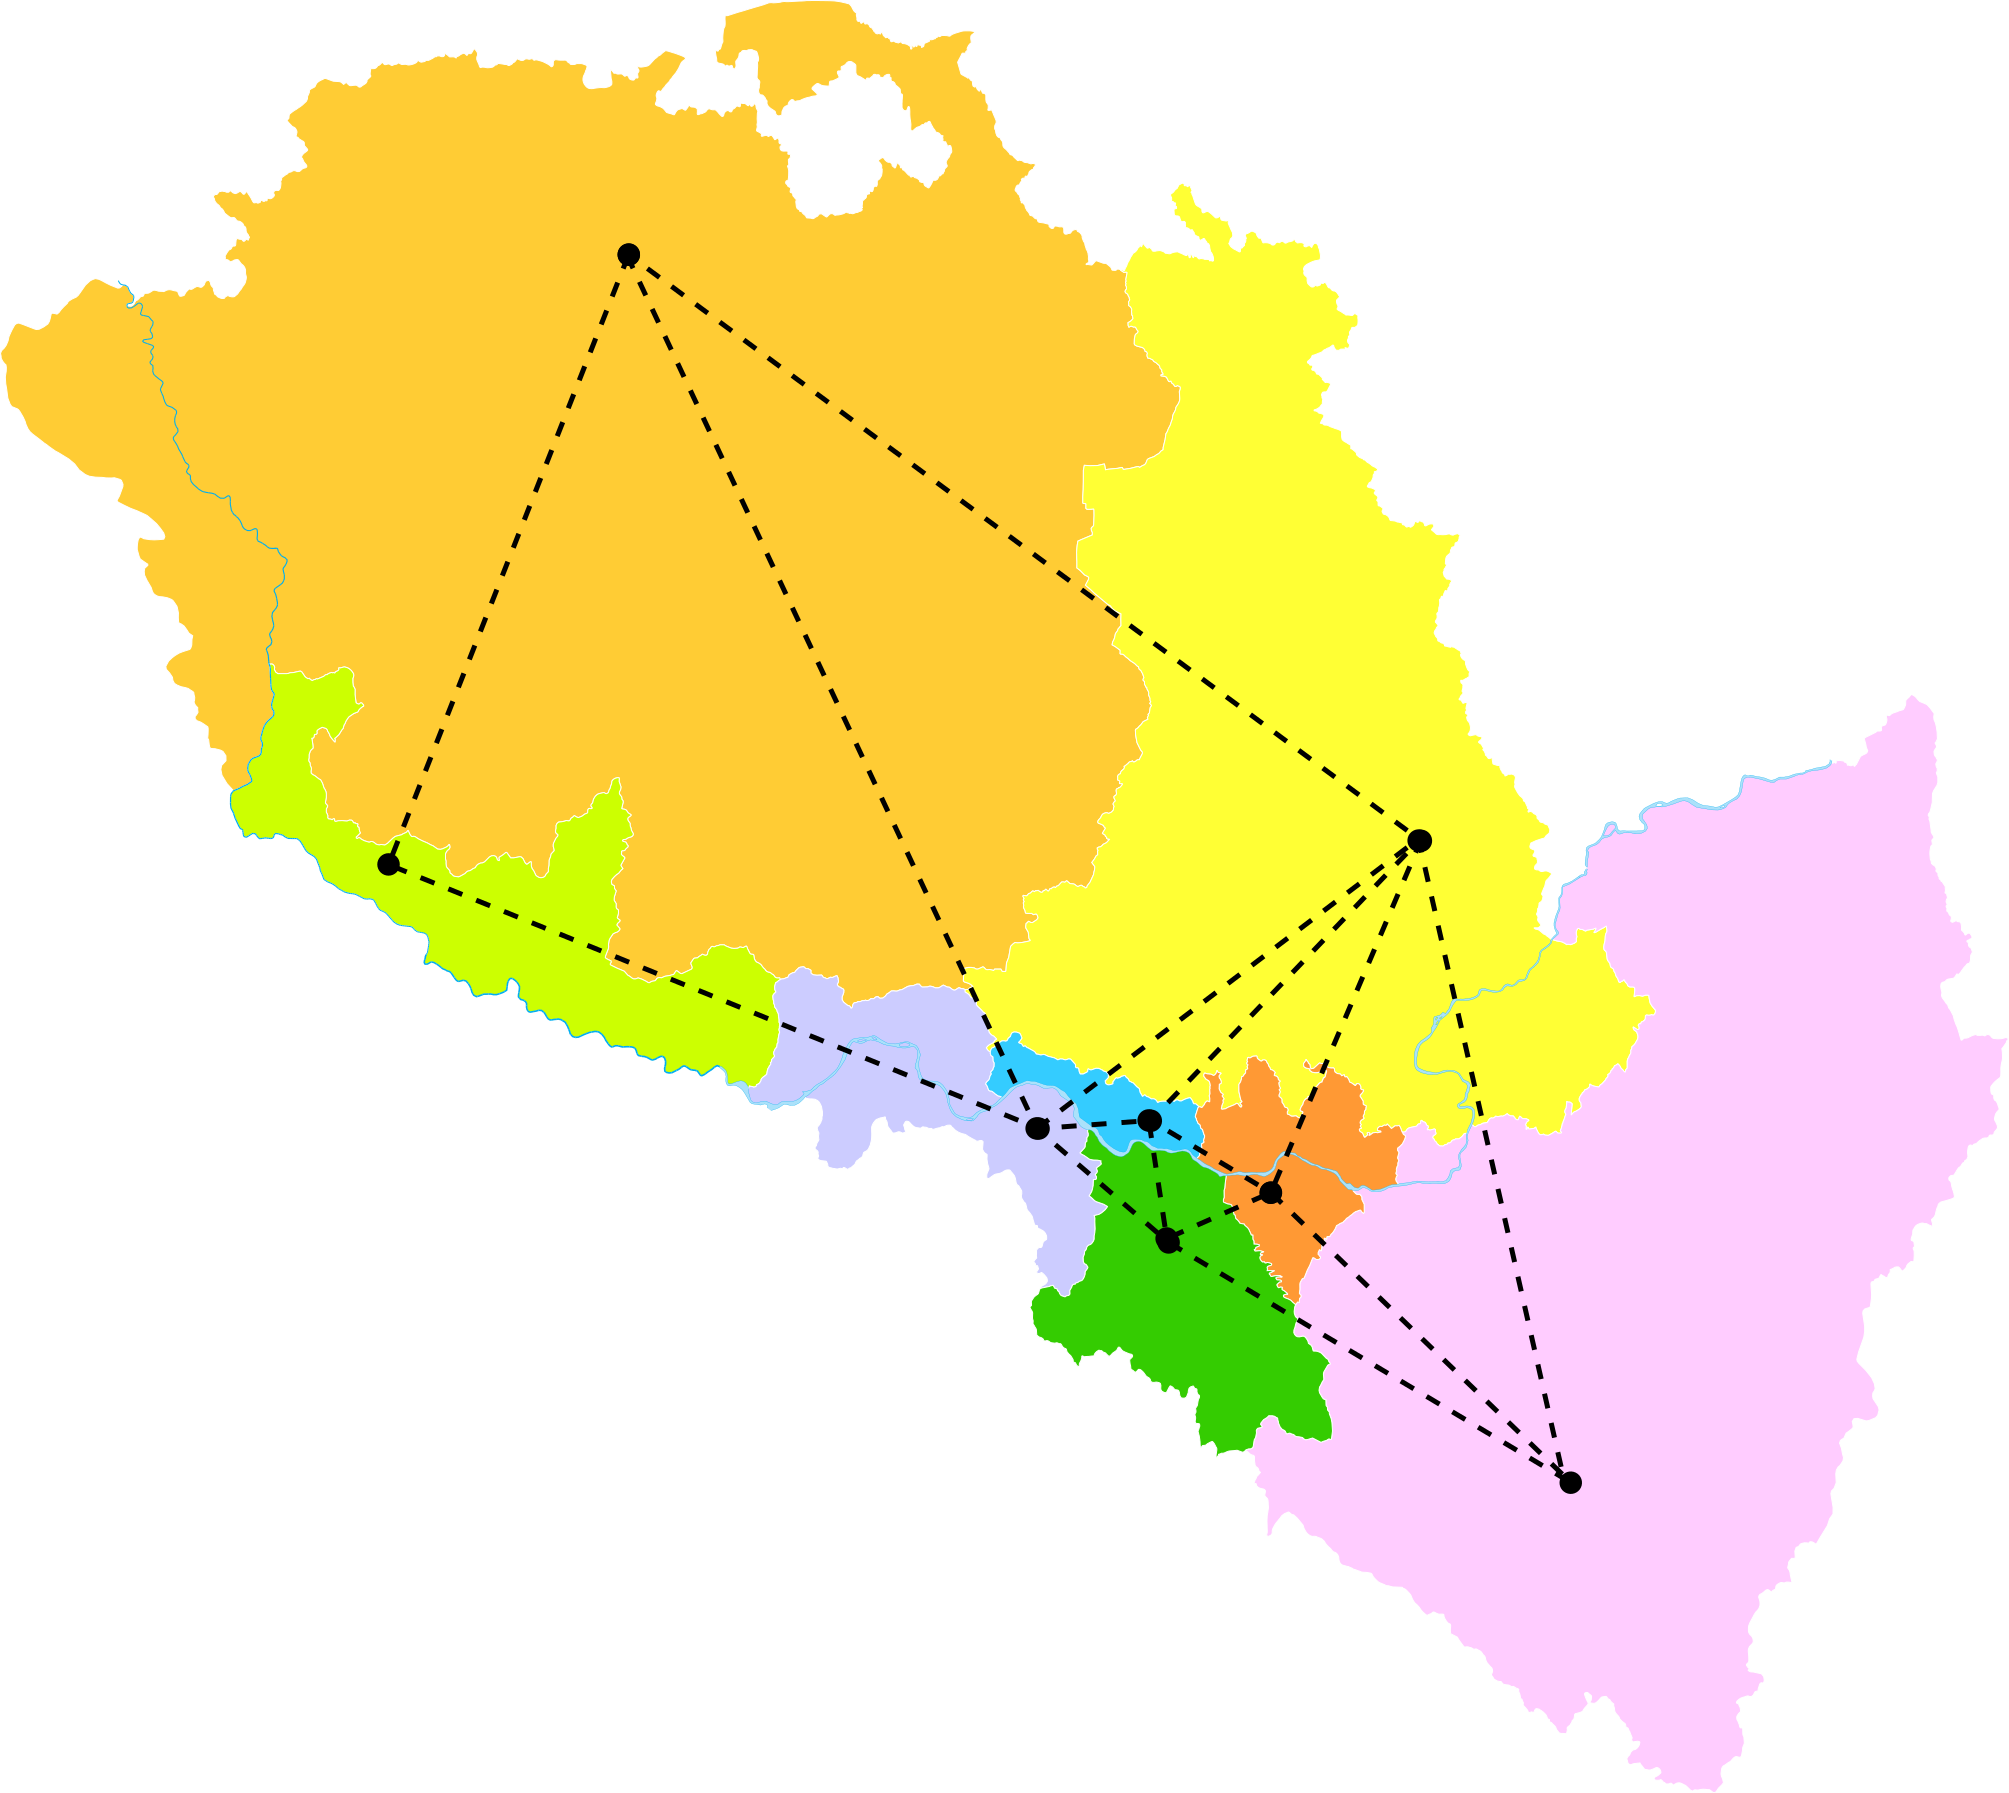
\includegraphics[width=0.5\textwidth]{Lanzhou.png}
			\caption{兰州市地图}
	\end{center}\end{figure}

	\begin{Exercises}
		\item 造访兰州. \begin{hint} 低碳出行, 请乘坐火车. \end{hint}
		\item 造访祁连山.
	\end{Exercises}

	% % % % % % % % % %
	\appendix
	\chapter{杂项 \texorpdfstring{$a+b$}{a+b}}
	按惯例, 附录以字母编号.
	
	\section{文字测试}
	龚自珍, \emph{乙亥杂诗}:
	\begin{enumerate}
		\item 其一
		\begin{center}
			掌故罗胸是国恩,小胥脱腕万言存。\\
			他年金匮如收采,来叩空山夜雨门。
		\end{center}
		\item 其二
		\begin{center}
			九州生气恃风雷,万马齐喑究可哀。\\
			我劝天公重抖擞,不拘一格降人才。
		\end{center}
		\item 其三
		\begin{center}
			吟罢江山气不灵,万千种话一灯青。\\
			忽然搁笔无言说,重礼天台七卷经。
		\end{center}
	\end{enumerate}	\index{gongzizhen@龚自珍}

	\begin{definition-theorem}[龚自珍]
		 《己卯京师作杂诗二首》:
		 \begin{center}
		 	文格渐卑庸福近,不知庸福究何如? \\
		 	常州庄四能怜我,劝我狂删乙丙书。
		 \end{center}
	\end{definition-theorem}

	交叉参照: 引理 \ref{prop:chen}.

	\section{测试: \texorpdfstring{$B_n(X)$}{BnX}}\label{sec:B}
	首先介绍 Bernoulli 多项式. 多项式变元记为 $X$.
	\begin{definition-proposition}\index{Bernoulli 多项式 (Bernoulli polynomials)}
		\emph{Bernoulli 多项式} $B_n(X) \in \mathbb{Q}[X]$ 由生成函数
		\begin{equation}
			\frac{t e^{tX}}{e^t - 1} = \sum_{n \geq 0} B_n(X) \cdot \frac{t^n}{n!} \; \in \mathbb{Q}[X][\![t]\!]
		\end{equation}
		确定. 称 $B_n := B_n(0)$ 为第 $n$ 个 \emph{Bernoulli 数}.
	\end{definition-proposition}

	\subsection{一张表格}
	以下来测试表格.

	\begin{table}[h!]
		\begin{equation*}\begin{array}{c|cccccccc}
			n & 0 & 1 & 2 & 4 & 6 & 8 & 10 & 12 \\ \hline
			B_n & 1 & -\frac{1}{2} & \frac{1}{6} & -\frac{1}{30} & \frac{1}{42} & -\frac{1}{30} & \frac{5}{66} & \frac{-691}{2730}
		\end{array}\end{equation*}
		\caption{前几个 Bernoulli 常数.}
		\label{table:B}
	\end{table}
	交叉参照: 练习 \ref{exo:Euler}.

	\begin{conjecture}[周恩来, 1917]\index{zhouenlai@周恩来}
		大江歌罢掉头东,邃密群科济世穷。面壁十年图破壁,难酬蹈海亦英雄。
	\end{conjecture}

	\begin{hypothesis}
		Riemann $\zeta$ 函数的非平凡零点全在 $\Re(s) = \frac{1}{2}$ 上.
	\end{hypothesis}

	引用测试: \cite{Oxl11, ZG}

	% % % % % % % % % %
	\backmatter
	% 使用 bibLaTeX 制作书目
	\printbibliography[heading=bibintoc]
	
	% 图, 表索引. 可有可无.
	\listoffigures
	\listoftables

	% 制作索引 (用 imakeidx 的功能可以制作多份)
	{\footnotesize
	\indexprologue{中文术语按汉语拼音排序.}
	\printindex}
\end{document}
